\chapter{The nature of accreted halo populations in the Milky Way}
\section{Modelling \mgfe{} as a function of \feh{}}
\label{sec:appA}
In order to test whether a change in slope is found in the relationship
between \mgfe{} and \feh{} in the identified accreted halo groups in Chapter \ref{chapter:highe},
I use a Bayesian inference to fit a piecewise-linear model to the
data. The form of the piecewise-linear function is given in
Equation~\ref{eq:pwlin}. I follow the general procedure outlined
in Section 7 of \citet{2010arXiv1008.4686H} for fitting models to
data with two-dimensional uncertainties. For completeness, I
re-iterate the mathematics here. The best fitting model is found
by maximising the likelihood function for the parameters $O =
[\mathrm{[Fe/H]}_0, \mathrm{[Mg/Fe]}_0, \theta_1, \theta_2]$ given
the data, which I assume here to be of the form
\begin{equation}
\ln{\mathcal{L}(O|\mathrm{[Fe/H]}, \mathrm{[Mg/Fe]})} = K -
\sum^{N}_{i=1}\left (\frac{\Delta_i^2}{2\Sigma^2_i} + \ln |\Sigma^{2}_i|\right)
\end{equation} 
where $\Delta_i^2$ defines the distance between the data-point $i$
and the model, and $\Sigma^2_i$ is the variance orthogonal to the
model, determined by the covariance matrix of the data points. $K$
is a normalisation constant, which is not necessary to consider in
the optimisation. I assume uninformative, flat priors on $\theta_{[1,2]}$,
and allow $\mathrm{[Fe/H]}_0$ and $\mathrm{[Mg/Fe]}_0$ to be free.
In this case, $\Delta_i^2$ is defined by
\begin{equation}
\label{eq:delta}
\Delta_i^2 = \hat{\bf{v}}^T \bf{Z}_i - \it{b} \cos\theta_{[1,2]}
\end{equation}
where $\bf{Z}_i$ is the column vector made by (\mgfe{},\feh{}$)_i$,
and $\hat{\bf{v}}$ is the unit vector orthogonal to the model:
\begin{equation}
\hat{\bf{v}} =
\frac{1}{\sqrt{1+m_{[1,2]}^2}}\begin{bmatrix}-m_{[1,2]}\\1\end{bmatrix} =
\begin{bmatrix}-\sin\theta_{[1,2]}\\\cos\theta_{[1,2]} \end{bmatrix}
\end{equation}
where $\theta_{[1,2]}$, here and in Equation \eqref{eq:delta}, is
the angle between the linear model at that \feh{} and the x-axis,
which is equal to $\arctan{m_{[1,2]}}$. $\Sigma^2_i$ is then simply
defined as the projection of the data-point's covariance matrix
$\bf{S}_i$ orthogonal to the model at that \feh{}
\begin{equation}
\Sigma^2_i = \hat{\bf{v}}^T \bf{S}_i \hat{\bf{v}}.
\end{equation}
In this case, I assume that the uncertainties on \mgfe{} and \feh{}
are uncorrelated, such that
\begin{equation}
\bf{S}_i = \begin{bmatrix} \delta \mathrm{[Fe/H]}_i & 0 \\ 0 & \delta \mathrm{[Mg/Fe]}_i \end{bmatrix}
\end{equation}
where I use the APOGEE catalogue values for the uncertainties on \feh{}
and \mgfe{}. I minimise the negative log-likelihood using a downhill
simplex algorithm \citep{doi:10.1093/comjnl/7.4.308}, and use this
optimal solution to initiate an Markov Chain Monte Carlo (MCMC)
sampling of the posterior PDF of the parameters O using an
affine-invariant ensemble MCMC sampler \citep{goodmanweare2010} as
implemented in the python package \texttt{emcee}
\citep{2013PASP..125..306F}. Finally, I report the median and standard
deviation of this posterior PDF as the best-fit parameters.

\section{Numerical Convergence Tests}
\label{sec:appB}
I examine in this appendix the effect on the results presented in Figures
\ref{fig:eagle} and \ref{fig:echange} of varying the simulation
resolution, box-size, and subgrid model parameters, in order to
demonstrate that these results are well converged numerically. I
perform the equivalent analysis to that presented for Recal-L025N752
(in the main body of the paper) on lower resolution volumes of the
EAGLE simulations.

\citet{2015MNRAS.446..521S} define `weakly' converged predictions
as those which are unaffected by variation in the simulation
resolution after re-calibrating the sub-grid physics. I test for this level of convergence
by examining the equivalently sized, $L=25$ cMpc, lower resolution
run (at a factor of 10 lower in mass than Recal-L025N752) which
adopts the `Reference' sub-grid model, which I refer to as
Ref-L025N376. The resulting equivalent of \ref{fig:eagle}
for Ref-L025N356 is shown in \ref{fig:n356ref}. It is clear from this figure
that the general prediction of \ref{fig:eagle} holds, in spite of
the fact that the lower resolution simulation clearly does not
resolve galaxies at masses as low as Recal-L025N752. The upper
envelope of the distribution, which defines the maximum $z=0$
eccentricity of a satellite merged at any given $z$, is still clear
out to $z\sim5$. Given that the sub-grid feedback model is adjusted
between the `Reference' and `Recalibrated' models to maintain the
predictions of the former, from this I conclude that the result is
`weakly' converged.

\begin{figure}
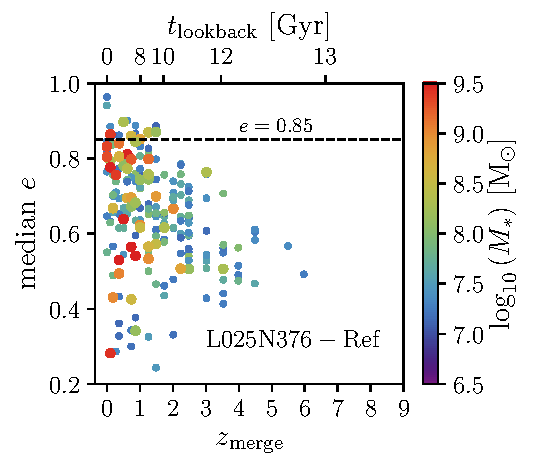
\includegraphics[width=0.5\columnwidth]{L025N376_REF_zmerge_mediane_npart20.pdf}
\caption[A recreation of Figure \ref{fig:eagle} for haloes in the Ref-L025N356 simulation]{\label{fig:n356ref} The merger time $z_\mathrm{merge}$ of
satellites accreted onto Milky Way mass haloes in the Ref-L025N356
simulation against the median eccentricity $e$ of their stellar
debris at $z=0$, produced via an equivalent analysis to that which
produced Figure \ref{fig:eagle}. The trends in Figures \ref{fig:n356ref}
and \ref{fig:eagle} are clearly conserved under an increase in
resolution with no recalibration of the sub-grid feedback model,
demonstrating the strong numerical convergence of these results.}
\end{figure}

In order to check that the prediction of EAGLE for the $z=0$
eccentricity as a function of merger time is `strongly' converged,
it is also necessary to ascertain that the trends in Figure \ref{fig:n356ref}
are conserved when the simulation resolution is increased, but the sub-grid
model held fixed. I test this by performing an equivalent analysis
on the Ref-L025N752 model, which has a resolution equal to the
Recal-L025N752 model, but assumes the same sub-grid physics as
Ref-L025N376. The resulting $z=0$ $e$ against merger time is shown
in Figure \ref{fig:n752ref}. The trends which are seen in both the
low-resolution `Reference' model (Figure \ref{fig:n356ref}) and
high-resolution `Recalibrated' model (Figure \ref{fig:eagle} in the
main text) are clearly conserved here also\footnote{ There is a very slight change in the exact position of the maximum of the distribution as a function of $z_\mathrm{merge}$, however, I contend that this is due to the stochastic sampling of the true underlying distribution.}, demonstrating the
`strong' numerical convergence of these results.

\begin{figure}
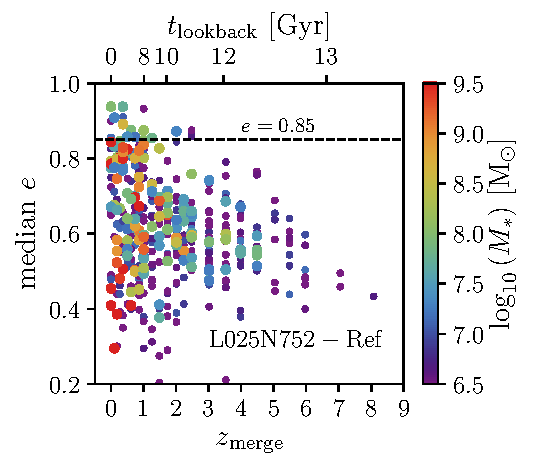
\includegraphics[width=0.5\columnwidth]{L025N752_REF_zmerge_mediane_npart20.pdf}
\caption[The equivalent of Figure \ref{fig:eagle} for haloes in the Ref-L025N752 simulation]{\label{fig:n752ref} The merger time $z_\mathrm{merge}$ of
satellites accreted onto Milky Way mass haloes in the Ref-L025N752
simulation against the median eccentricity $e$ of their stellar
debris at $z=0$, produced via an equivalent analysis to that which
produced Figure \ref{fig:eagle}. The upper envelope of $z=0$
eccentricity for a given merger time is reproduced in this lower
resolution simulation, albeit with a different calibration of the
subgrid model, demonstrating the `weak' convergence of this result.}
\end{figure}


\begin{figure}
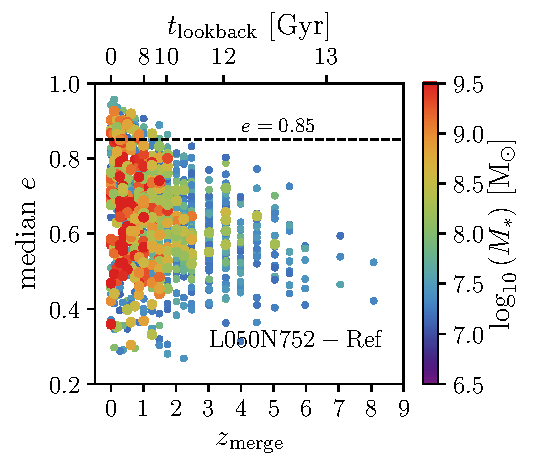
\includegraphics[width=0.5\columnwidth]{L050N752_REF_zmerge_mediane_npart20.pdf}
\caption[The equivalent of Figure \ref{fig:eagle} for haloes in the Ref-L050N752 simulation]{\label{fig:l50} The merger time $z_\mathrm{merge}$ against
median eccentricity $e$ of the stellar debris at $z=0$, of the 1154
accreted satellites (with $> 20$ particles) of 126 central galaxies
from the Ref-L050N752 simulation, produced via an equivalent analysis
to that which produced Figure \ref{fig:eagle}. The trends seen in
Figures \ref{fig:eagle}, \ref{fig:n356ref} and \ref{fig:n752ref}
are seen again, even though a much larger sample of accretion events
is analysed.} \end{figure}

I also perform the analysis on a larger volume, $L=50$ cMpc, EAGLE
simulation, which adopts the `Reference' sub-grid model at the same resolution as the smaller volume: Ref-L050N752.
In this much larger volume, I
track the accretion of 1154 satellites onto 126 central haloes,
again with halo masses which are roughly equivalent to that of the
Milky Way. The resulting distribution of satellite debris in median
$e(z=0)$  against merger time is shown in Figure \ref{fig:l50}.
Again, the trend between the maximum $z=0$ eccentricity and
$z_\mathrm{merge}$ is seen, now more clearly, as a result of the
better statistics offered by the increased sample size. This
demonstrates that the results presented from EAGLE are strongly
robust to variations in the simulation resolution, box-size and
sub-grid physics.

Finally, I show in Figure \ref{fig:echange_lowres} that the findings
of Figure \ref{fig:echange} are robust to degradation in the
simulation resolution. It is possible that the dynamical interaction
between the central galaxy and the accreting satellite may be poorly
modelled by the simulations, which are of a relatively low resolution
\citep[as opposed to idealised simulations such as those of
e.g.][]{2017MNRAS.464.2882A}, reducing the action of the central
galaxy on the accreting satellites. By this reasoning, a degradation
in the simulation resolution should decrease any changes to the
orbital properties of the satellites, as these effects would be
worsened. In Figure \ref{fig:echange}, showing the higher resolution
simulation, I find the scatter around the dashed unity line to be
0.13. At the lower resolution adopted by Ref-L025N376, I find the scatter to be comparable,
if not slightly increased - at 0.15. As a result, I contend that
these interactions are likely well modelled by the simulation, even
at this relatively low resolution.

\begin{figure}
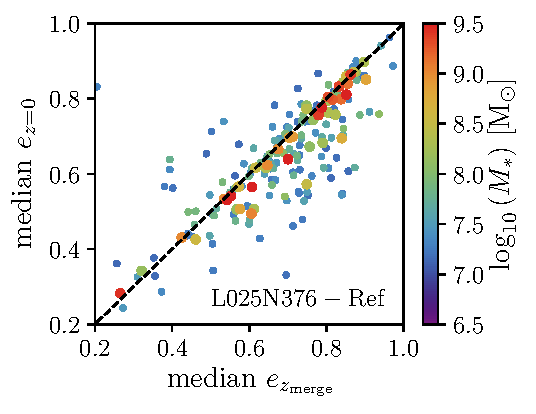
\includegraphics[width=0.5\columnwidth]{L025N376_REF_inite_mediane_npart20.pdf}
\caption[A recreation of Figure \ref{fig:echange} using satellites accreted onto Milky Way mass haloes in the lower resolution Ref-L025N376 simulation]{\label{fig:echange_lowres} The change in eccentricity between the snapshot immediately after the satellites become unbound and $z=0$ in the L025N376-Ref simulation (equivalent to Figure \ref{fig:echange} in the main text). Degrading the simulation resolution has little effect on this result, which suggests that the lack of any significant radialisation or circularisation of orbits after satellite infall is not due to poorly resolved dynamics, which would act to reduce any scatter upon degradation of the simulation resolution.  }
\end{figure}

